\section{Máquina Virtual}
\label{sec:maquina-virtual}

A máquina virtual utilizada é baseada na arquitetura de máquina virtual
\sctt{secd} descrita por Peter Landin\cite{secd} com pequenas alterações nos
registradores e instruções propostas por Kent Dybvig em sua tese de
doutorado\cite{3imp}. Esta, como a de Landin, utiliza uma estrutura baseada em pilha,
com um pequeno número de registradores que apontam para memória organizada em
listas encadeadas. Uma curiosidade interessante: de acordo com algumas fontes
\cite{craig:vm} a máquina \sctt{secd} pode ser considerada a primeira máquina
virtual já especificada, embora sua primeira implementação tenha ocorrido apenas
anos depois.

A estrutura da máquina é bastante simples: cinco registradores e 14 instruções.
Os registradores são todos baseados em memória organizada como listas, enquanto
que as instruções, em sua maioria, compartilham uma peculiaridade: Recebem como parâmetro
o código que deverá ser executado ao fim da instrução em questão. Algumas
exceções óbvias são as instruções \sctt{halt}, que termina a operação da
máquina e obviamente não recebe código algum para continuar, e \sctt{test}, que
decide entre duas linhas diferentes e portanto recebe dois parâmetros de código
para escolher executar ao fim da mesma.

Esta propriedade de representar o fluxo de controle de instruções
explícitamente na forma de parâmetros para todas as instruções simplifica
significativamente a implementação de duas das mais complexas funcionalidades
da linguagem: A obrigatoriedade de eliminar as chamadas terminais e a criação e
aplicação de continuações em tempo de execução.

Levando-se em consideração a simplicidade do código necessário para se
implementar a máquina virtual \sctt{secd} (aproximadamente 350 linhas de código
em C++) e o fato de ela tornar trivial a implementação das duas funcionalidades
mais complexas, esta foi escolhida para a implementação da fase de
interpretação propriamente dita neste interpretador. Nas seções
\ref{ss:registradores} e \ref{ss:instrucoes} são detalhados os registradores e
instruções que compõem esta máquina.

\subsection{Registradores}
\label{ss:registradores}

O estado interno da máquina é composto pelos seus cinco registradores: os
quatro originais descritos por Landin, que dão o nome à máquina (\sctt{stack},
\sctt{environment}, \sctt{code} e \sctt{dump}), acrescidos de um
\sctt{acumulador}.

\begin{itemize}

\item O registrador \sctt{stack}, que aponta para uma lista encadeada que
armazena temporariamente os valores intermediários que serão ser passados para
chamadas de funções como parâmetros. 

\item Na arquitetura original não havia a presença de um \sctt{acumulador}, que
foi utilizado apenas para simplificar a codificação de algumas etapas, e
poderia perfeitamente ser substituído pelo uso judicioso do topo da pilha para
esta função. Este serve apenas para guardar resultados intermediários de forma
separada da pilha de parâmetros guardada na \sctt{stack}. 

\item O registrador \sctt{environment} aponta para uma lista composta dos
níveis de vínculos de variáveis válidos no escopo atual, estendendo-se até que
o escopo global é atingido por último. São armazenados de forma encadeada, com
cada contexto possuindo um ponteiro para o contexto no qual foi criado.

\item O registrador \sctt{code} aponta para uma representação da próxima
instrução a ser executada e pode ser visto como um análogo ao contador de
programa em uma arquitetura convencional de hardware, com a diferença que, no
modelo utilizado neste trabalho, cada instrução carrega consigo uma referência
explícita para a próxima instrução a ser executada, ao invés de depender de um
incremento implícito de contador.

\item O registrador \sctt{dump} mantém uma área de armazenamento temporário
para os outros registradores, exceto o \sctt{acumulador}, composto de um
conjunto \{\sctt{s}, \sctt{e}, \sctt{c}, \sctt{d}\} que, tendo como elemento o
conteúdo anterior do registrador \sctt{dump}, mantém uma pilha de contextos. É
internamente utilizado para manter a pilha de registros de ativação de chamadas
de função. 

\end{itemize}


\subsection{Representação visual dos Registradores}
\label{ss:registradores-visual}

Para atuar sobre o estado interno da máquina, são utilizadas 14 instruções que são
descritas a seguir. Na verdade, apenas 13 instruções seriam necessárias para
implementar a arquitetura proposta neste trabalho mas, devido a um problema de
projeto na fase do compilador uma instrução extra foi incluída de forma que a
máquina virtual possui algum conhecimento sobre o sistema de macros.

Durante a discussão das instruções a seguir, serão utilizadas as seguintes
representações para o conteúdo de cada registrador nos exemplos:

\begin{itemize}

\item Os registradores \sctt{stack} e \sctt{acumulador} serão representados
pela representação dos seus valores em Scheme
 com as seguintes adições:
 \begin{itemize}
 
 \item Closures serão representadas com o formato \texttt{closure(contexto;
parametros; corpo)}, em que \texttt{contexto} é representado como descrito
abaixo para o registrador \sctt{environment}, \texttt{parametros} é
representado como uma lista de átomos \textit{Scheme} e \texttt{corpo} é
representado como o descrito abaixo para o registrador \sctt{code}.

 \end{itemize}
\item Os contextos em \sctt{environment} serão representados por uma lista de
elementos delimitados por colchetes, em que o elemento mais à esquerda
representa o contexto mais recente. Elementos mais à direita indicam os demais
níveis de contextos no escopo atual, ou seja: \texttt{[a = 1, b = 2][c = 3][]}
representa o contexto em que as variáveis \texttt{a} e \texttt{b} têm valores
1, e 2, que é encadeado ao contexto em que \texttt{c} possui o valor 3. O
contexto vazio, \texttt{[]}, indica o escopo global com todos os vínculos
existentes neste.

\item O registrador \sctt{code} é representado pela notação de função
\textit{Scheme} com a exceção que parâmetros representados como palavras em
\sctt{maiúsculas} representam trechos de código da máquina virtual omitidos por
clareza.

\item O conteúdo de \sctt{dump} será representado usando a notação de cada um
dos registradores cujos valores armazena, delimitados por um par de chaves, com
registradores irrelevantes para o exemplo substituído por reticências. O
conteúdo de \sctt{dump} sem elementos será representado apenas como a lista
vazia \sctt{()}.

\end{itemize} 

Na figura \ref{fig:maquina} pode-se ver um exemplo da representação utilizada
para a máquina virtual como um todo durante a descrição das instruções a
seguir.

\begin{figure}[h!]
\centering
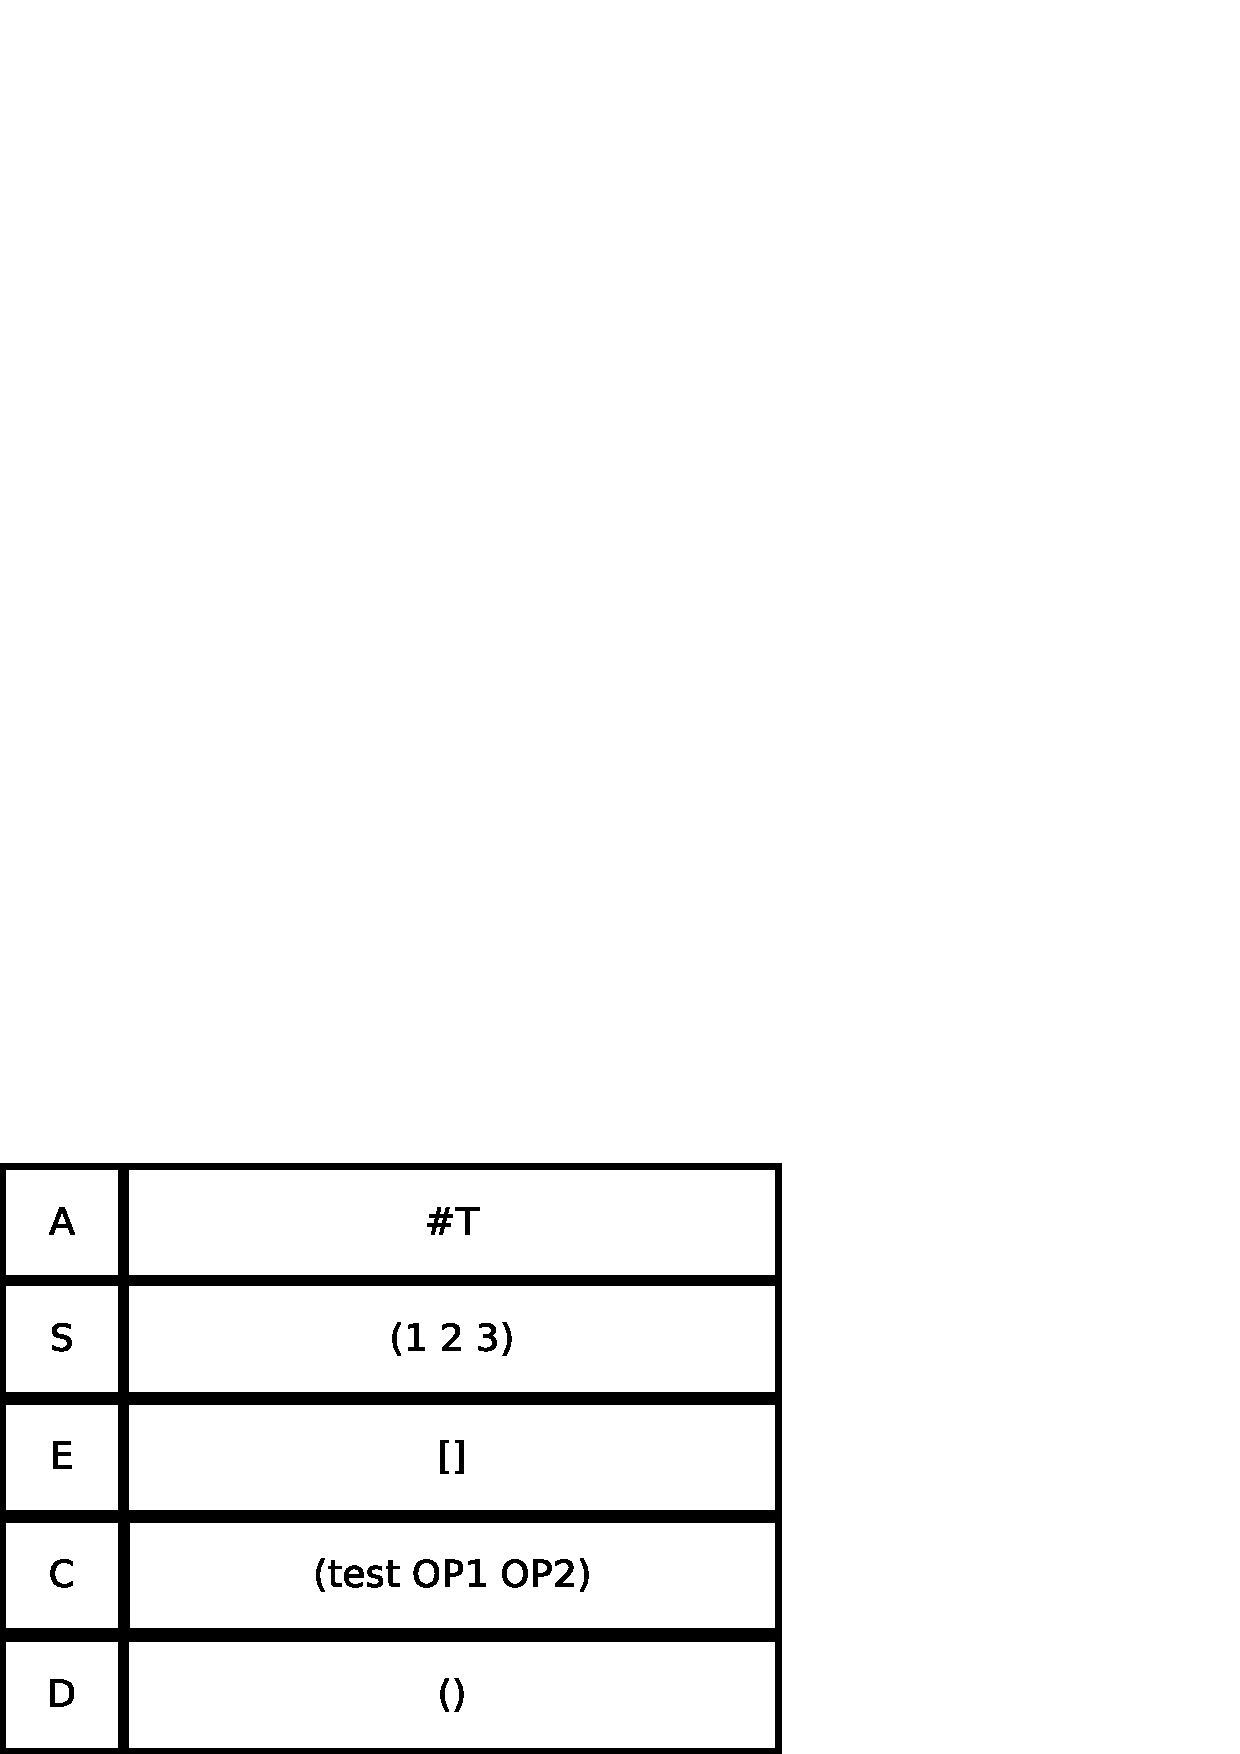
\includegraphics[width=.35\textwidth]{../images/maquina.pdf}
\caption{Estrutura da máquina quando da execução de uma instrução \sctt{test}}
\label{fig:maquina}
\end{figure}


\subsection{Instruções}
\label{ss:instrucoes}

A instrução \sctt{test} realiza controle de fluxo condicional, utilizando o
valor armazenado no \sctt{acumulador} e dois parâmetros chamados
\sctt{conseqüência} e \sctt{alternativa}. Ambos os parâmetros representam
trechos de código. Um exemplo de sua execução pode ser visto na figura
\ref{fig:op-test}

De acordo com o valor armazenado no \sctt{acumulador}, decide se deve continuar
a execução pela \sctt{consequência} (caso este valor seja diferente do literal
false) ou pela \sctt{alternativa} (caso este seja igual ao literal false),
armazenando no registrador \sctt{code} o valor escolhido entre os dois
parâmetros.

\begin{figure}[h!]
\centering
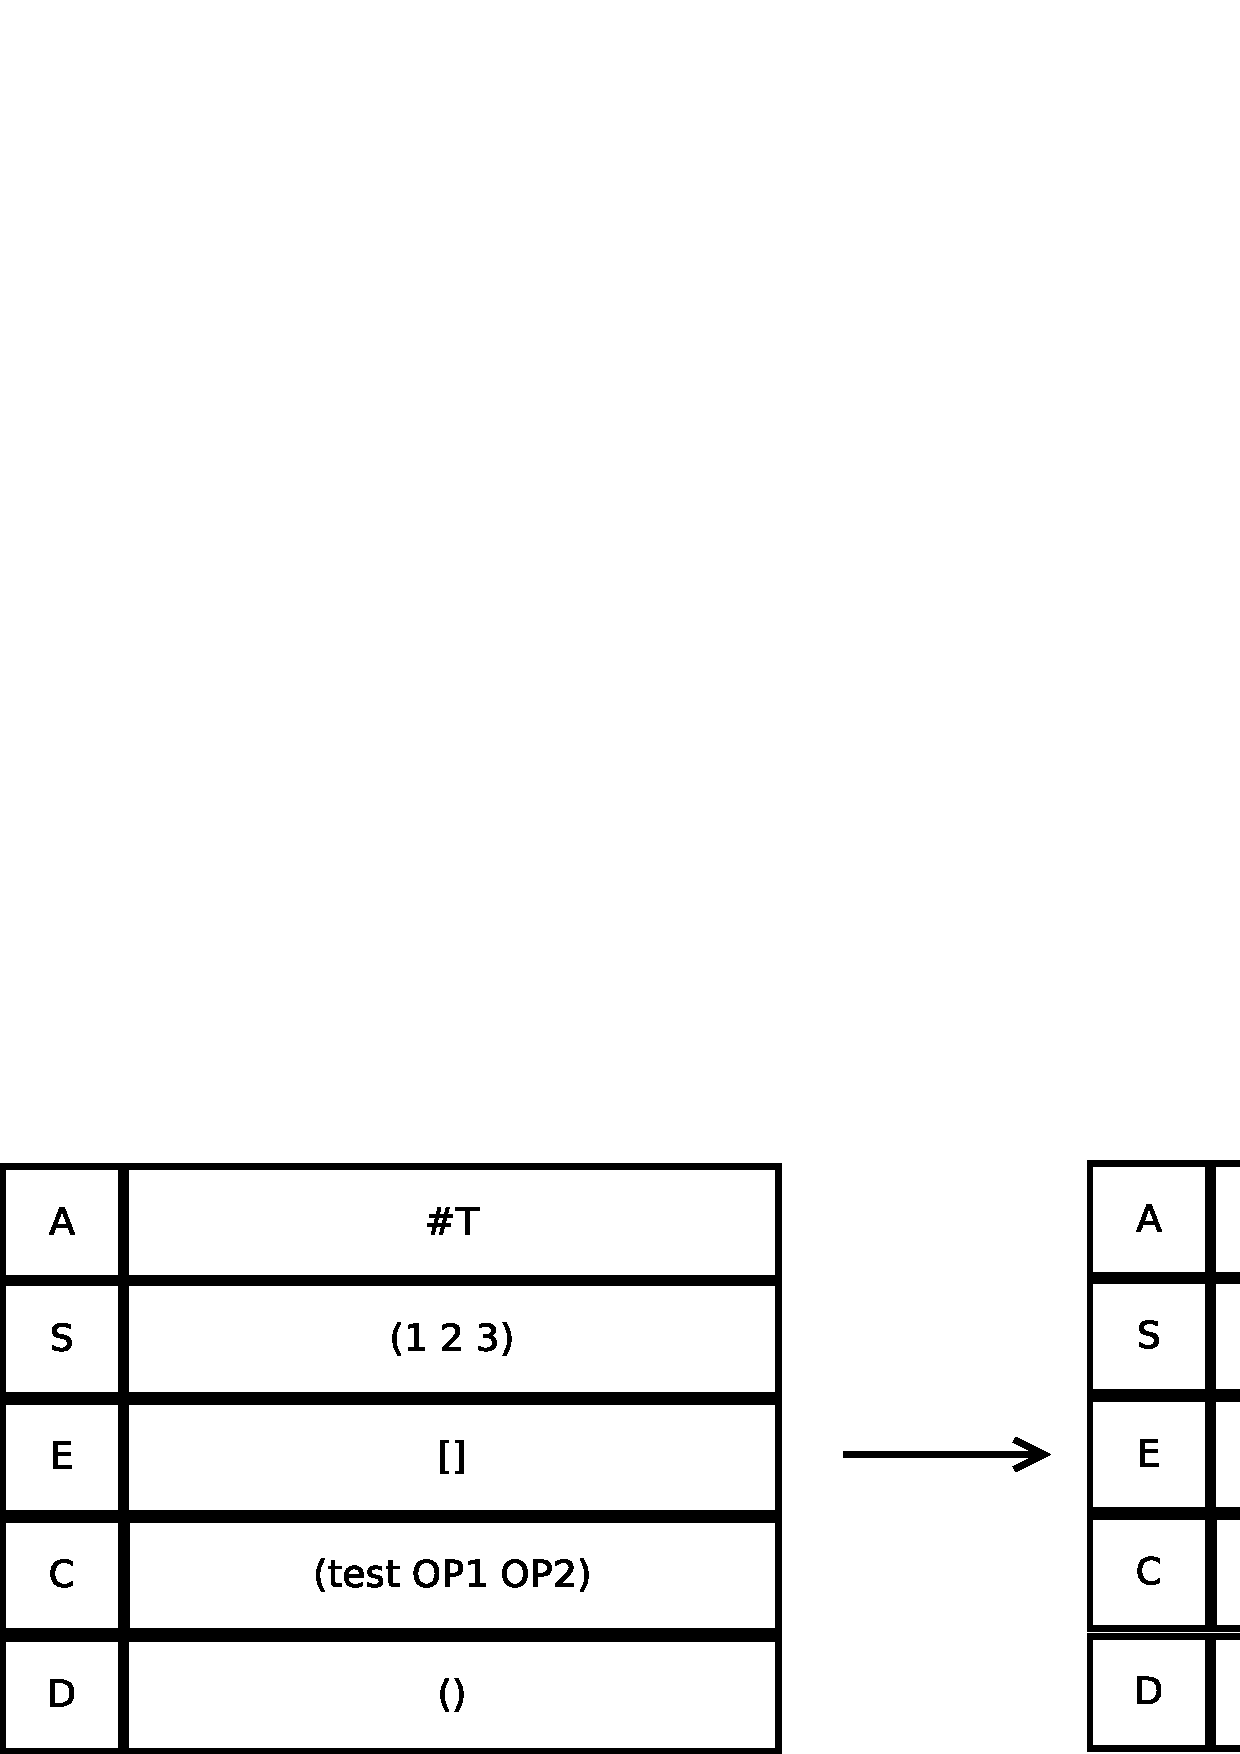
\includegraphics[width=.8\textwidth]{../images/op-test.pdf}
\caption{Comportamento da máquina ao executar uma instrução \sctt{test}}
\label{fig:op-test}
\end{figure}

A instrução \sctt{frame} é utilizada para salvar o estado da
máquina quando se faz necessária a execução de um outro procedimento,
armazenando o valor dos registradores atuais em uma pilha. Recebe dois
parâmetros: \sctt{retorno}, que indica o código que deve ser executado quando
este frame for restaurado, e \sctt{próximo}, que indica o código a ser
executado ao fim desta instrução.

Um novo frame é armazenado no registrador \sctt{dump}, contendo o valor dos
registradores \sctt{environment}, \sctt{stack} e \sctt{dump}, junto o valor do
parâmetro \sctt{retorno} que atua como valor do registrador \sctt{code} no
frame. Então o valor do registrador \sctt{stack} é setado para uma lista vazia
e o valor do registrador \sctt{code} é setado como o valor recebido no
parâmetro \sctt{próximo}. Um exemplo de sua execução pode ser visto na figura
\ref{fig:op-frame}.

A separação entre a instrução \sctt{frame} e a instrução \sctt{apply},
utilizada para invocar uma chamada de função, é crucial para a implementação da
eliminação de chamadas terminais: quando o compilador identifica que uma
chamada é terminal, simplesmente omite a criação de uma instrução \sctt{frame}.

\begin{figure}[h!]
\centering
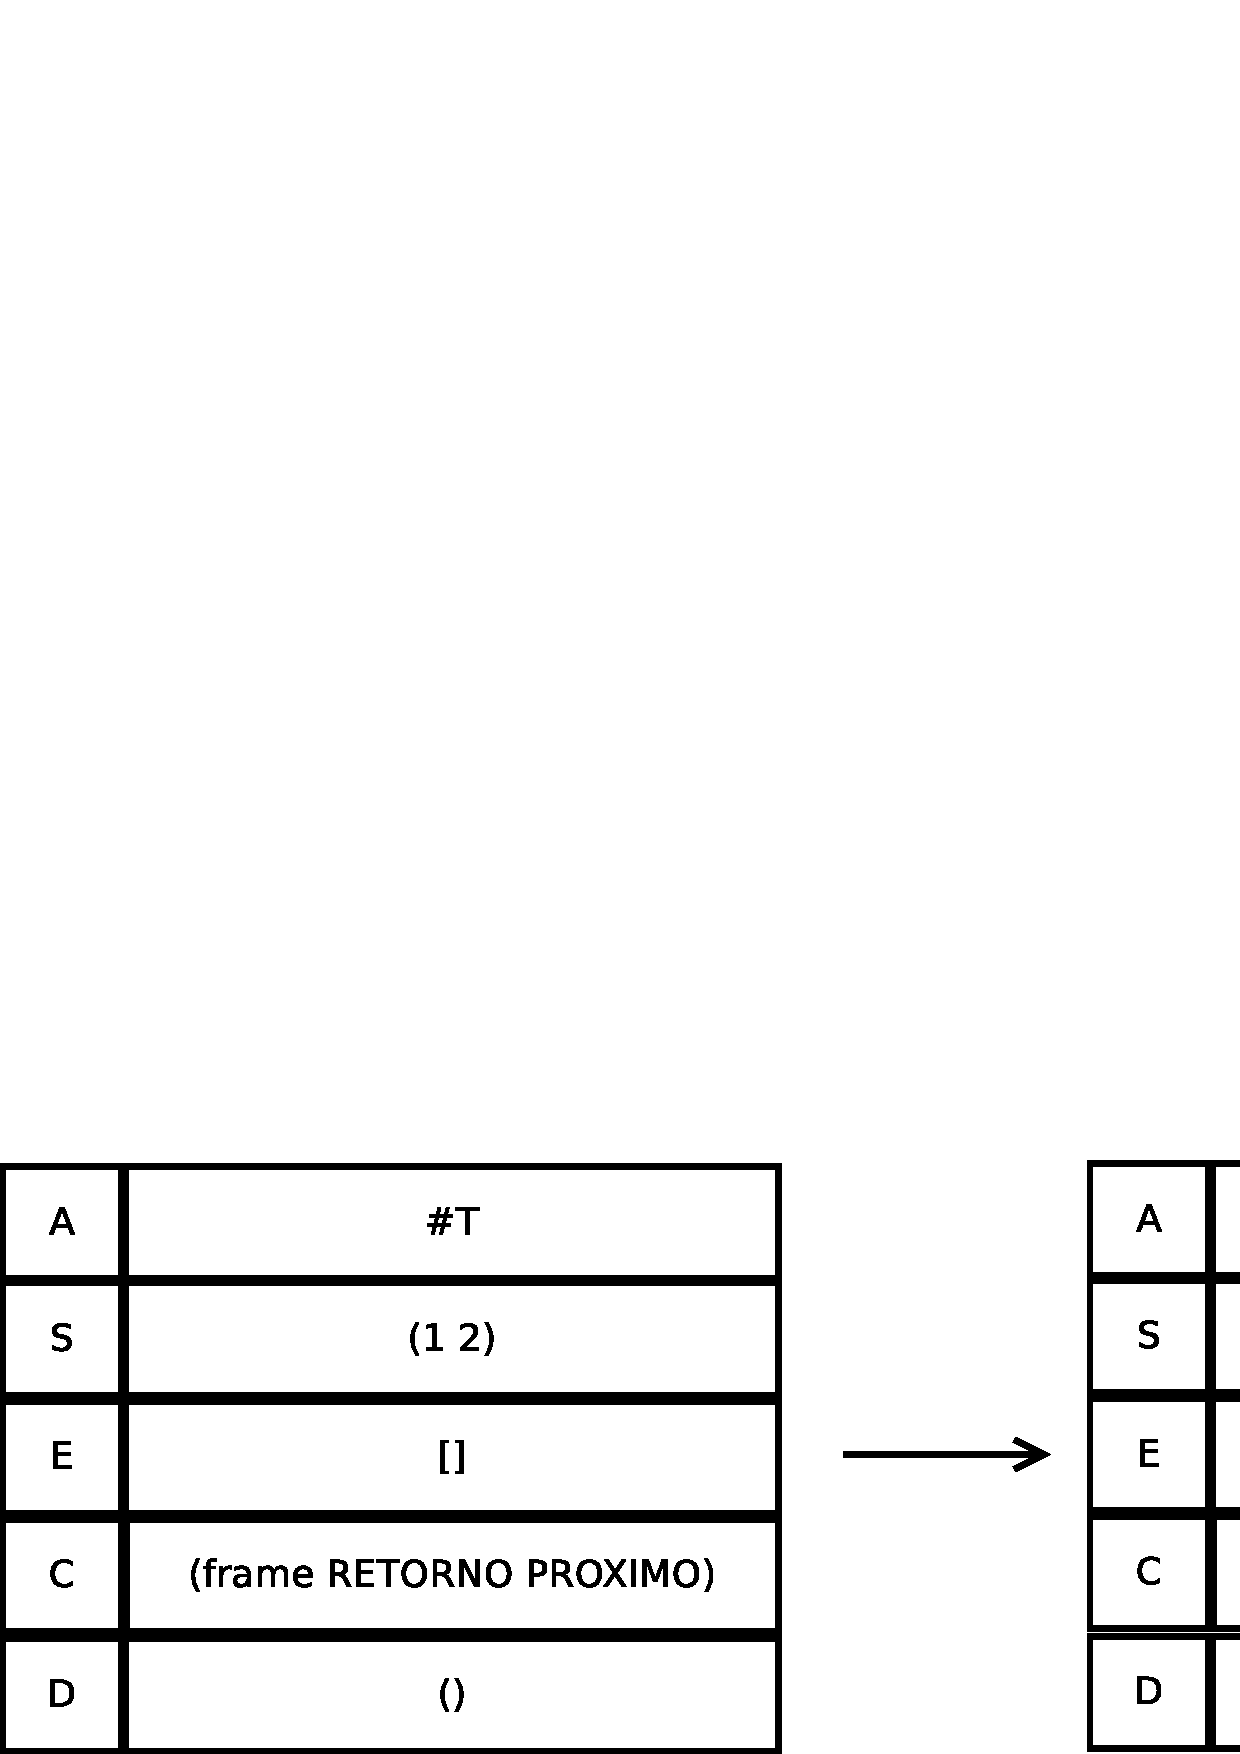
\includegraphics[width=.8\textwidth]{../images/op-frame.pdf}
\caption{Comportamento da máquina ao executar uma instrução \sctt{frame}}
\label{fig:op-frame}
\end{figure}


A instrução \sctt{constant}  carrega o valor de um literal
para utilização por outra instrução. Recebe dois parâmetros: \sctt{valor} e
\sctt{próximo}, que representam, respectivamente, o valor do literal a ser
carregado e o código a ser executado a seguir. O valor recebido como
\sctt{valor} substitui o valor no registrador \sctt{acumulador} e o valor em
\sctt{próximo} substitui o valor no registrador \sctt{code}. Um exemplo de sua execução pode ser visto na figura
\ref{fig:op-constant}.

\begin{figure}[h!]
\centering
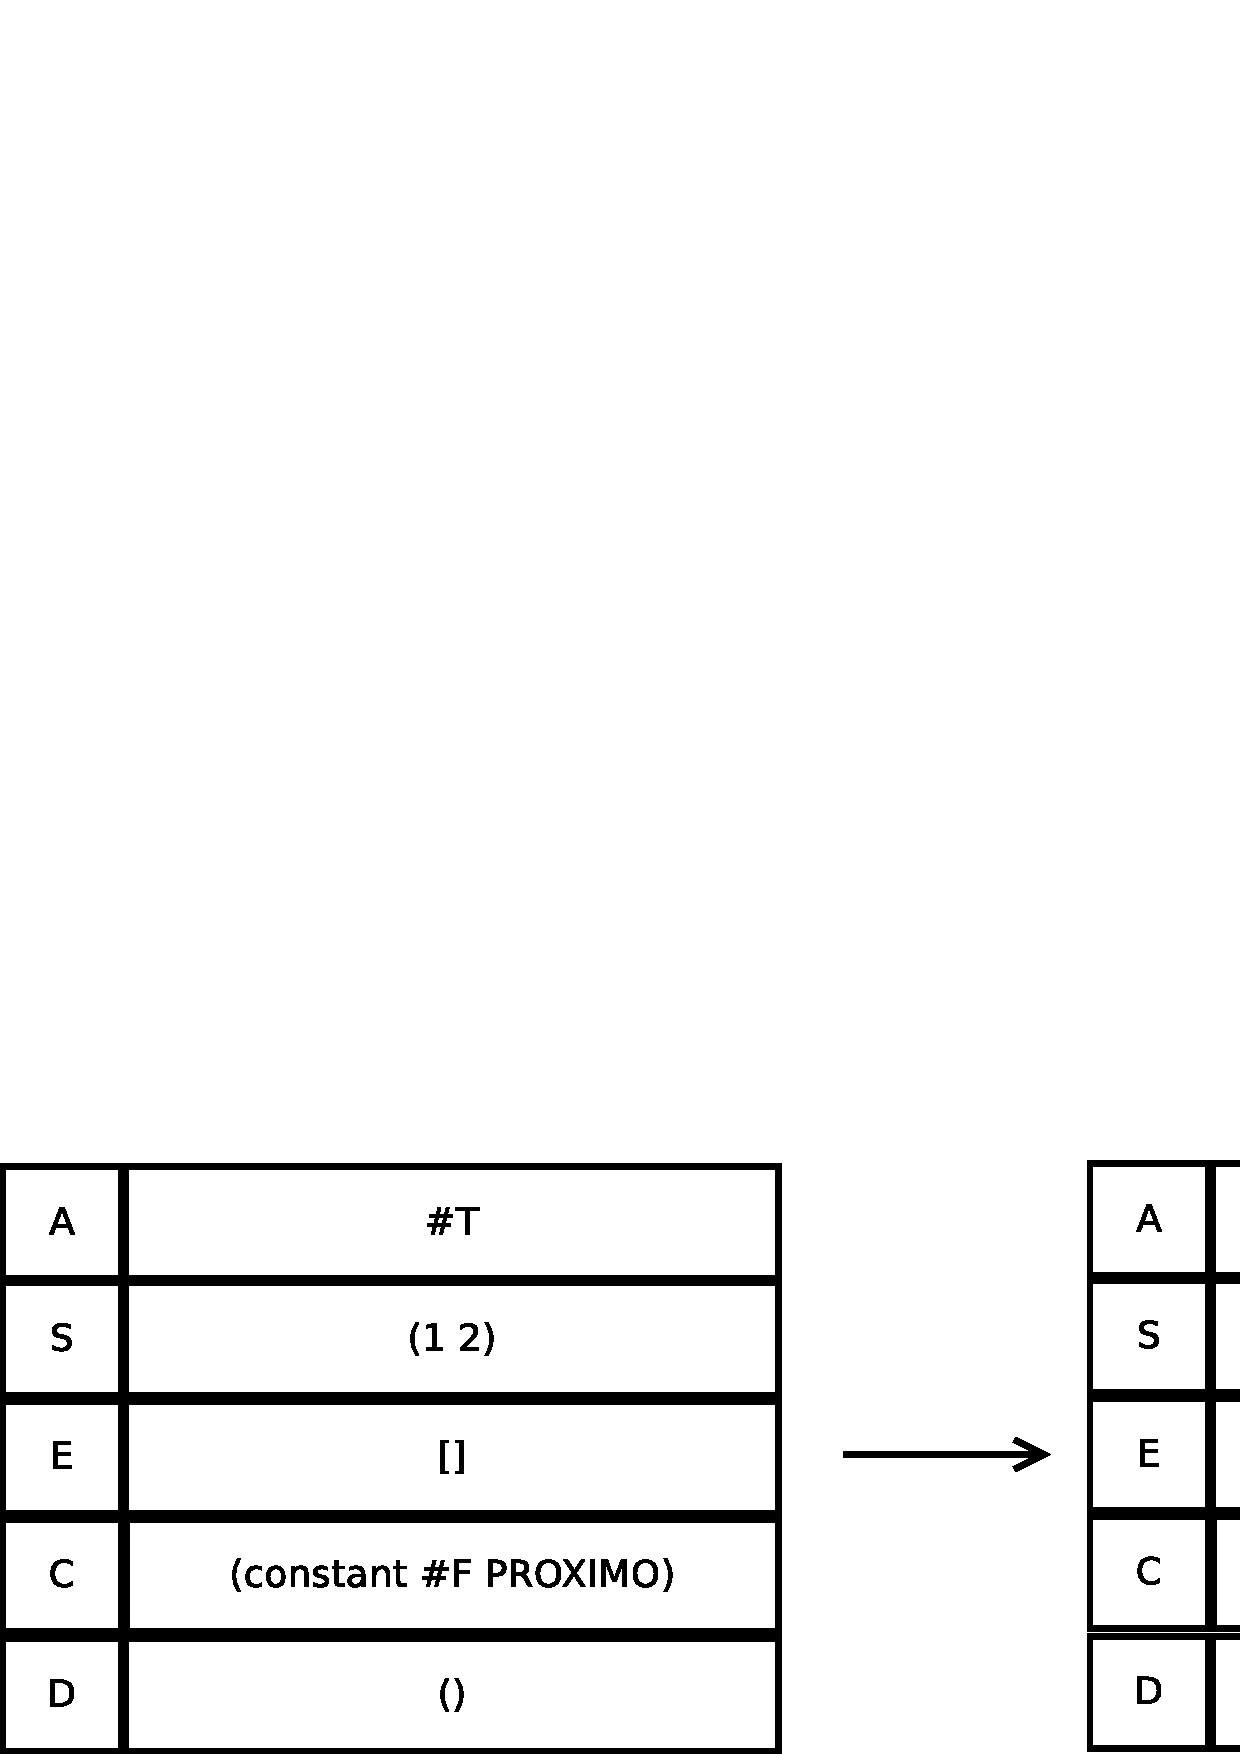
\includegraphics[width=.8\textwidth]{../images/op-constant.pdf}
\caption{Comportamento da máquina ao executar uma instrução \sctt{constant}}
\label{fig:op-constant}
\end{figure}


A instrução \sctt{lookup}  carrega o valor de uma variável
para o \sctt{acumulador}. Recebe dois parâmetros: \sctt{nome} e \sctt{próximo},
que representam o nome da variável a ser buscada e o código a ser executado a
seguir. O valor recebido como \sctt{nome} é utilizado para fazer a busca no
escopo de variáveis atual e o valor encontrado é então carregado no registrador
\sctt{acumulador}; o valor armazenado em \sctt{próximo} substitui o valor no
registrador \sctt{code}. Um exemplo de sua execução pode ser visto na figura
\ref{fig:op-lookup}.

\begin{figure}[h!]
\centering
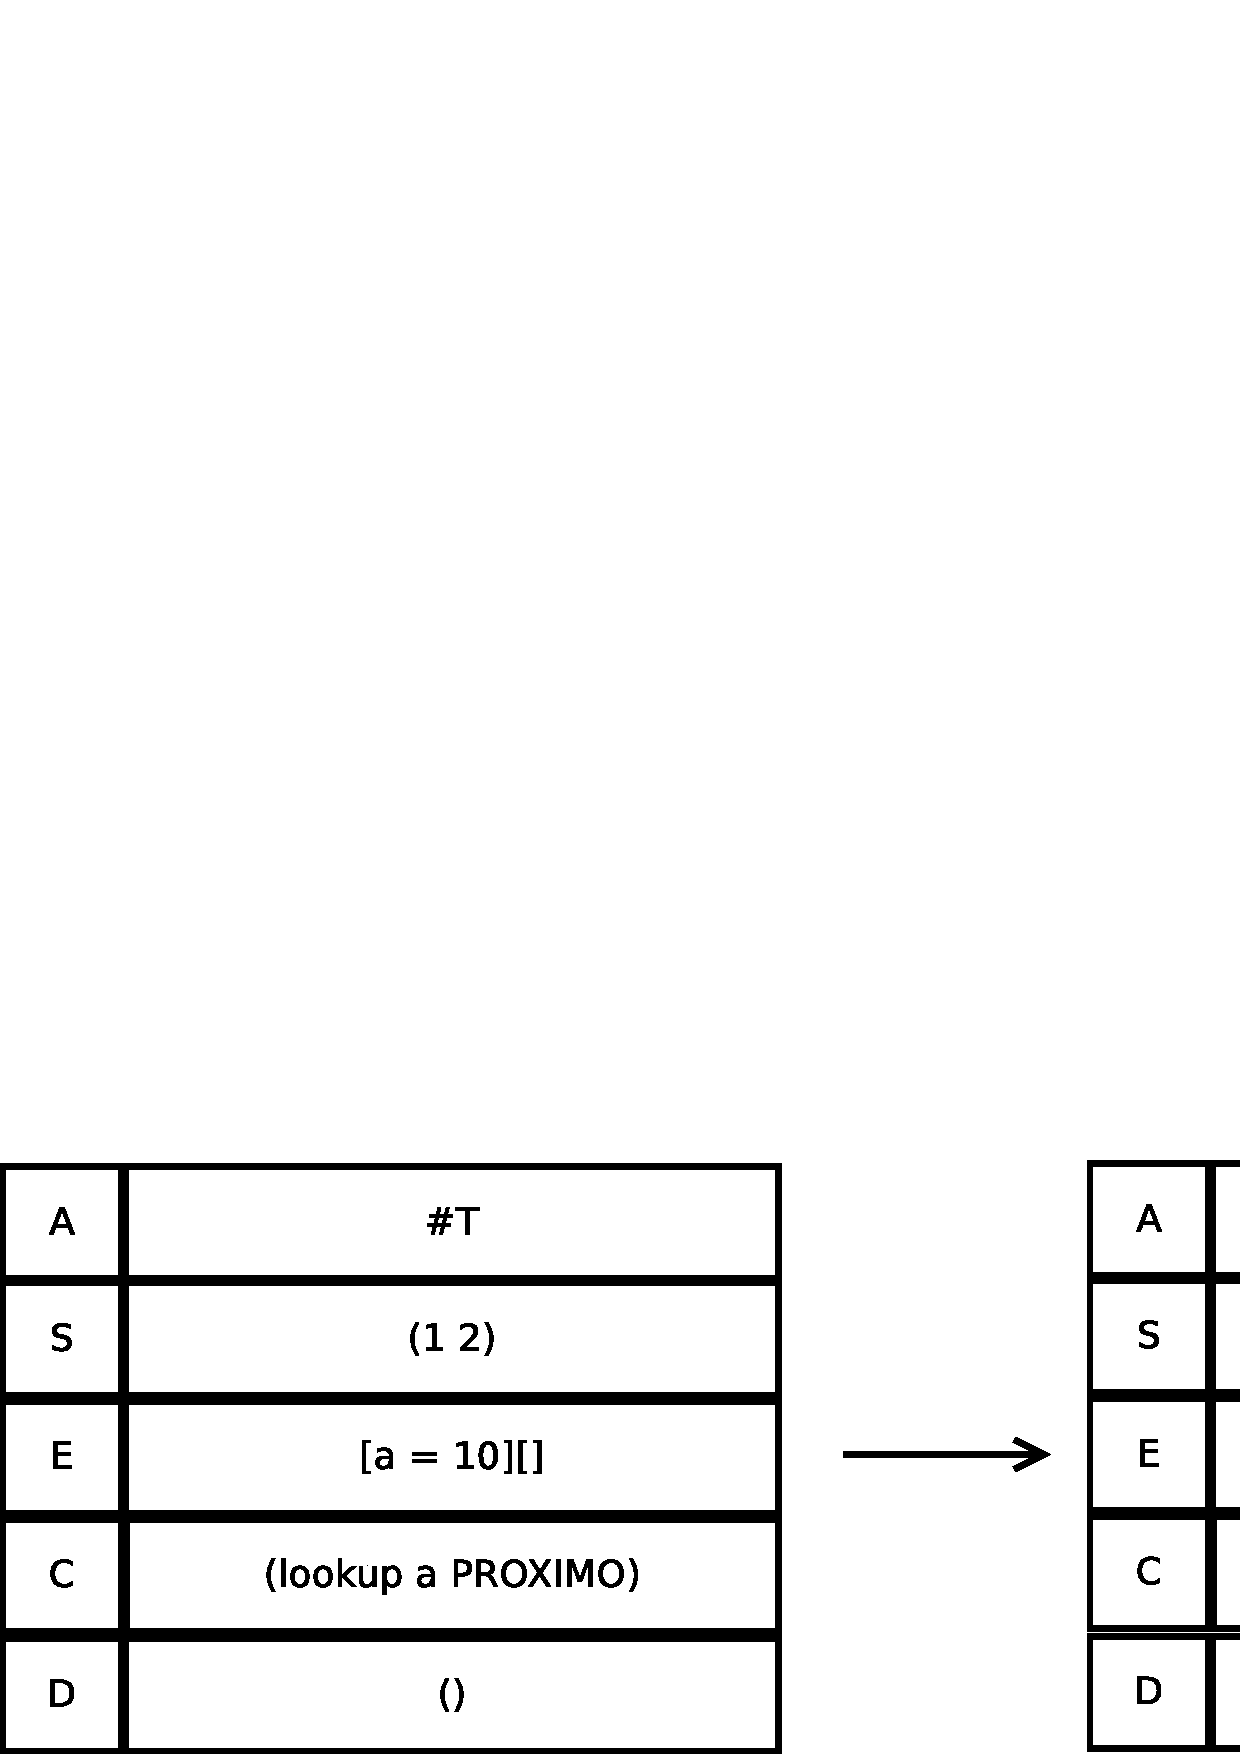
\includegraphics[width=.8\textwidth]{../images/op-lookup.pdf}
\caption{Comportamento da máquina ao executar uma instrução \sctt{lookup}}
\label{fig:op-lookup}
\end{figure}


A instrução \sctt{assign}  substitui o valor de uma variável
no escopo atual. Recebe dois parâmetros: \sctt{nome}, que representa o nome da
variável, e \sctt{próximo}, que indica o código a ser executado após a execução
da instrução atual. O valor da variável armazenada sob o vínculo indicado pelo
conteúdo de \sctt{nome} no escopo atual é substituído pelo valor no registrador
\sctt{acumulador}; caso não haja variável armazenada sob o nome indicado no
escopo atual, um erro é sinalizado.  O valor em \sctt{próximo} então substitui
o valor no registrador \sctt{code}. Um exemplo de sua execução pode ser visto na figura
\ref{fig:op-assign}.

\begin{figure}[h!]
\centering
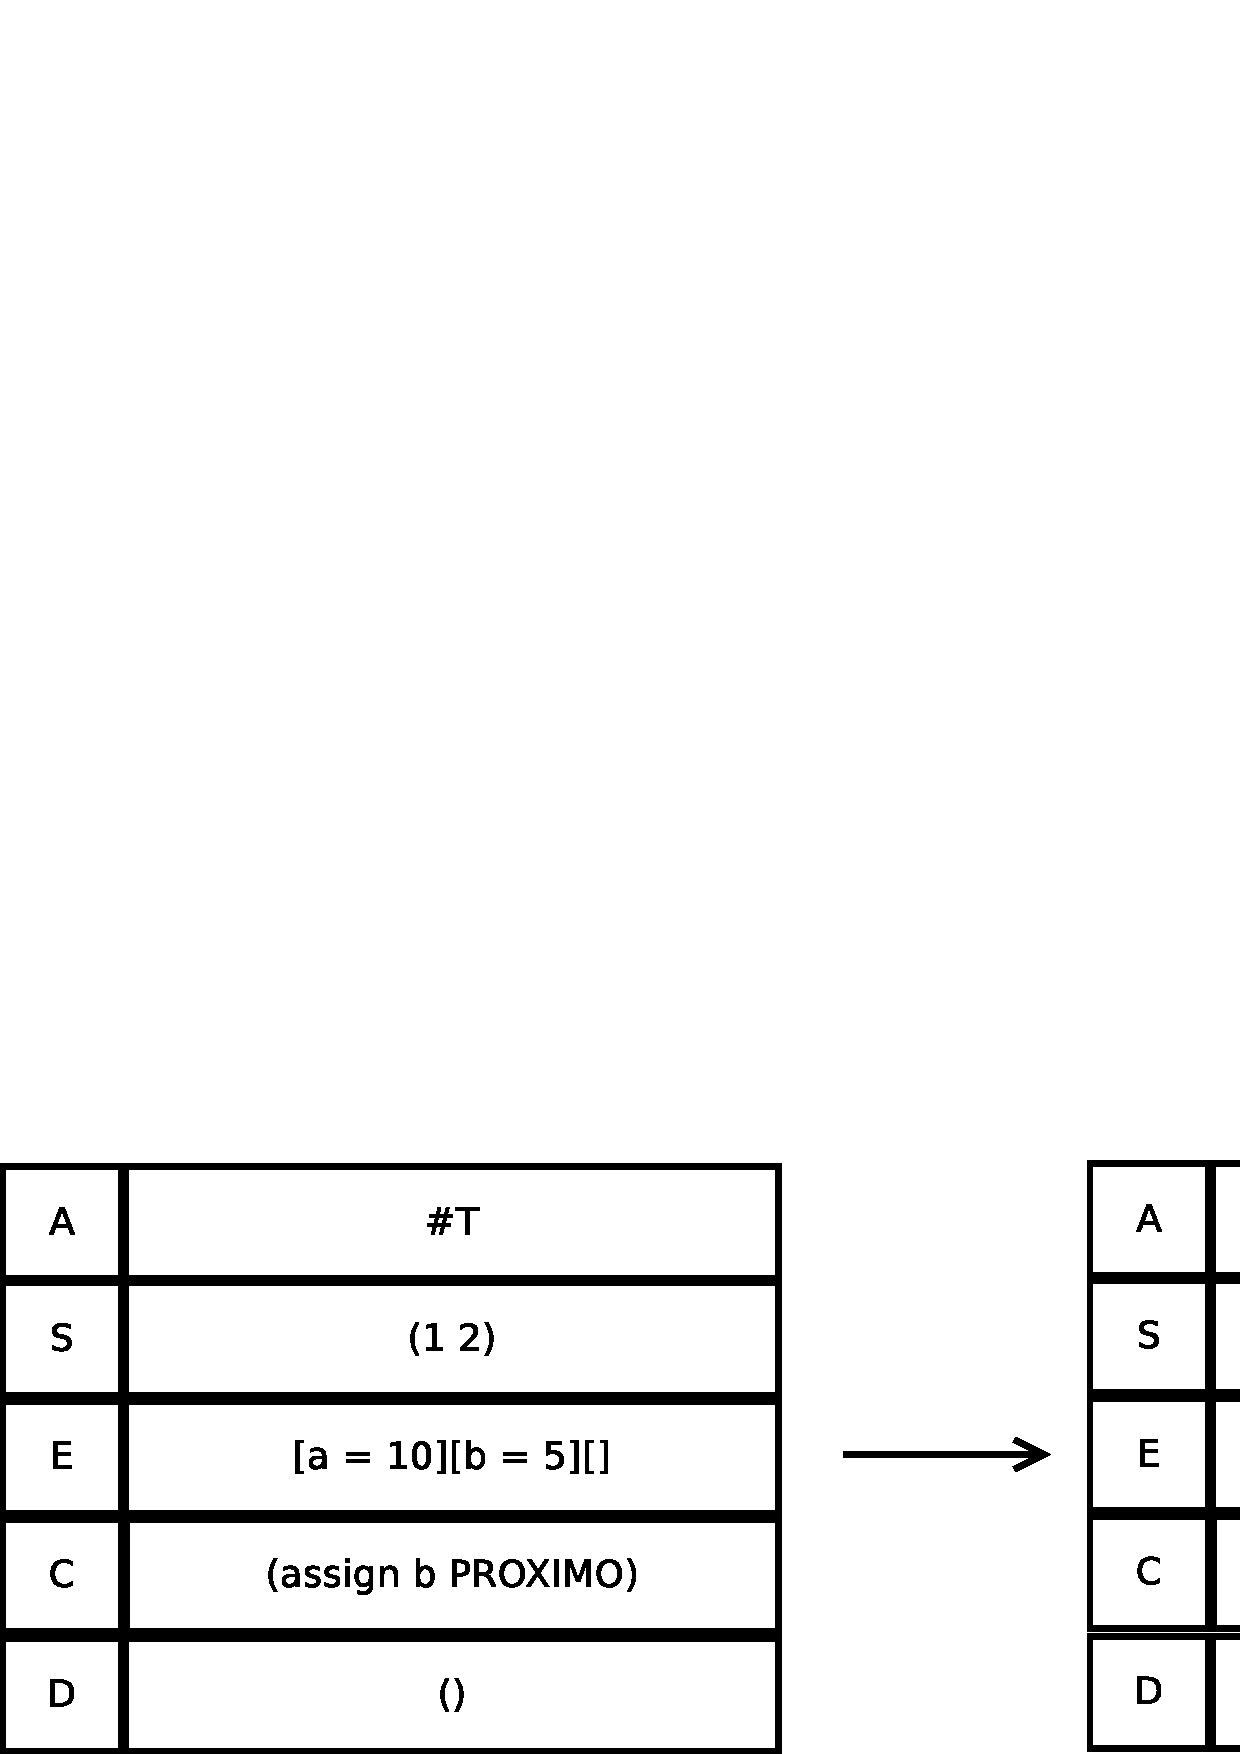
\includegraphics[width=.8\textwidth]{../images/op-assign.pdf}
\caption{Comportamento da máquina ao executar uma instrução \sctt{assign}}
\label{fig:op-assign}
\end{figure}


A instrução \sctt{bind}  cria, no nível mais próximo do escopo
atual, um novo vínculo de variável. Funciona de modo quase idêntico à instrução
\sctt{assign} recebendo os mesmos parâmetros, com a diferença que caso não haja
variável armazenada sob o nome indicado, uma variável é criada para conter o
valor. Um exemplo de sua execução pode ser visto na figura
\ref{fig:op-bind}.

\begin{figure}[h!]
\centering
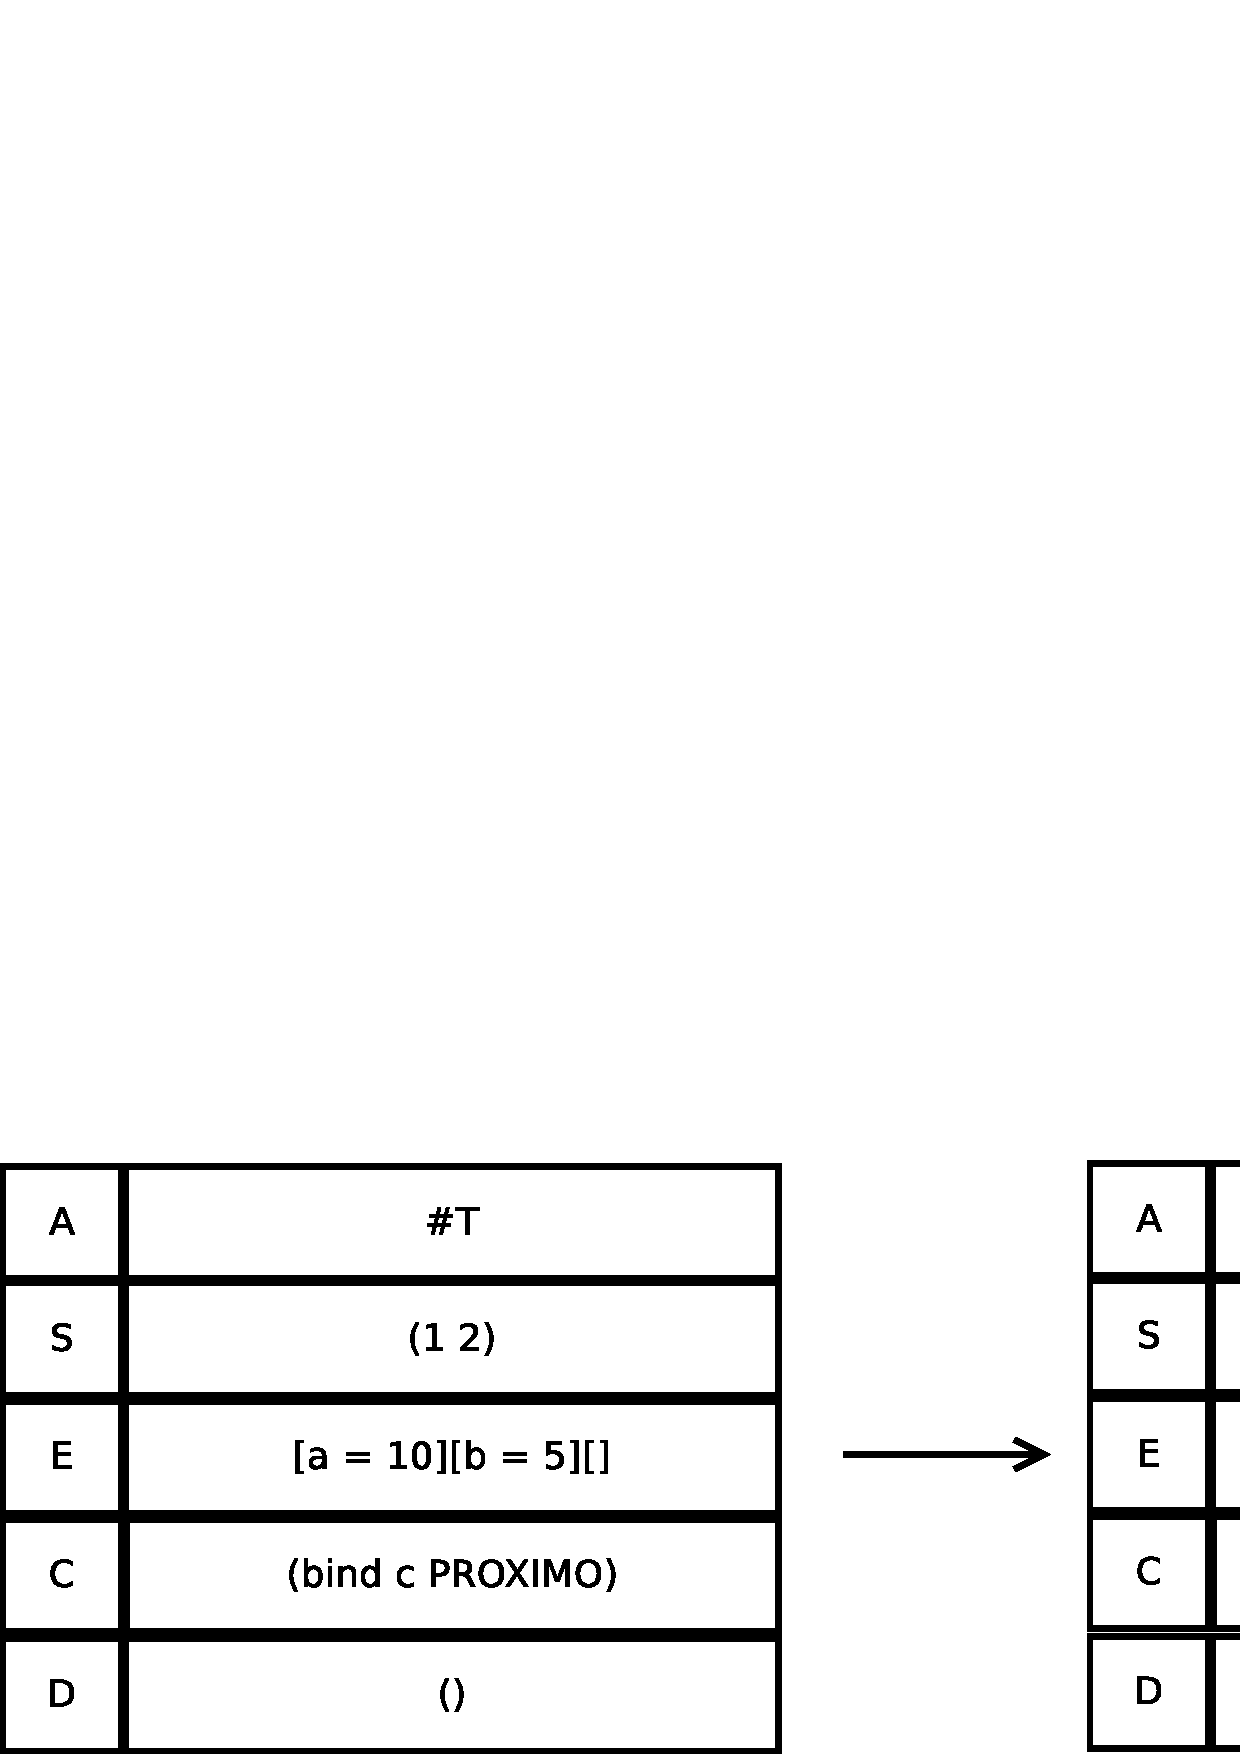
\includegraphics[width=.8\textwidth]{../images/op-bind.pdf}
\caption{Comportamento da máquina ao executar uma instrução \sctt{bind}}
\label{fig:op-bind}
\end{figure}


A instrução \sctt{argument}  armazena na pilha do
registrador \sctt{stack} o valor atual do \sctt{acumulador}. Recebe apenas o
parâmetro \sctt{próximo} indicando qual o código a ser executado a seguir, que
então é utilizado para configurar o registrador \sctt{code}.  Um exemplo de sua execução pode ser visto na figura
\ref{fig:op-argument}.


\begin{figure}[h!]
\centering
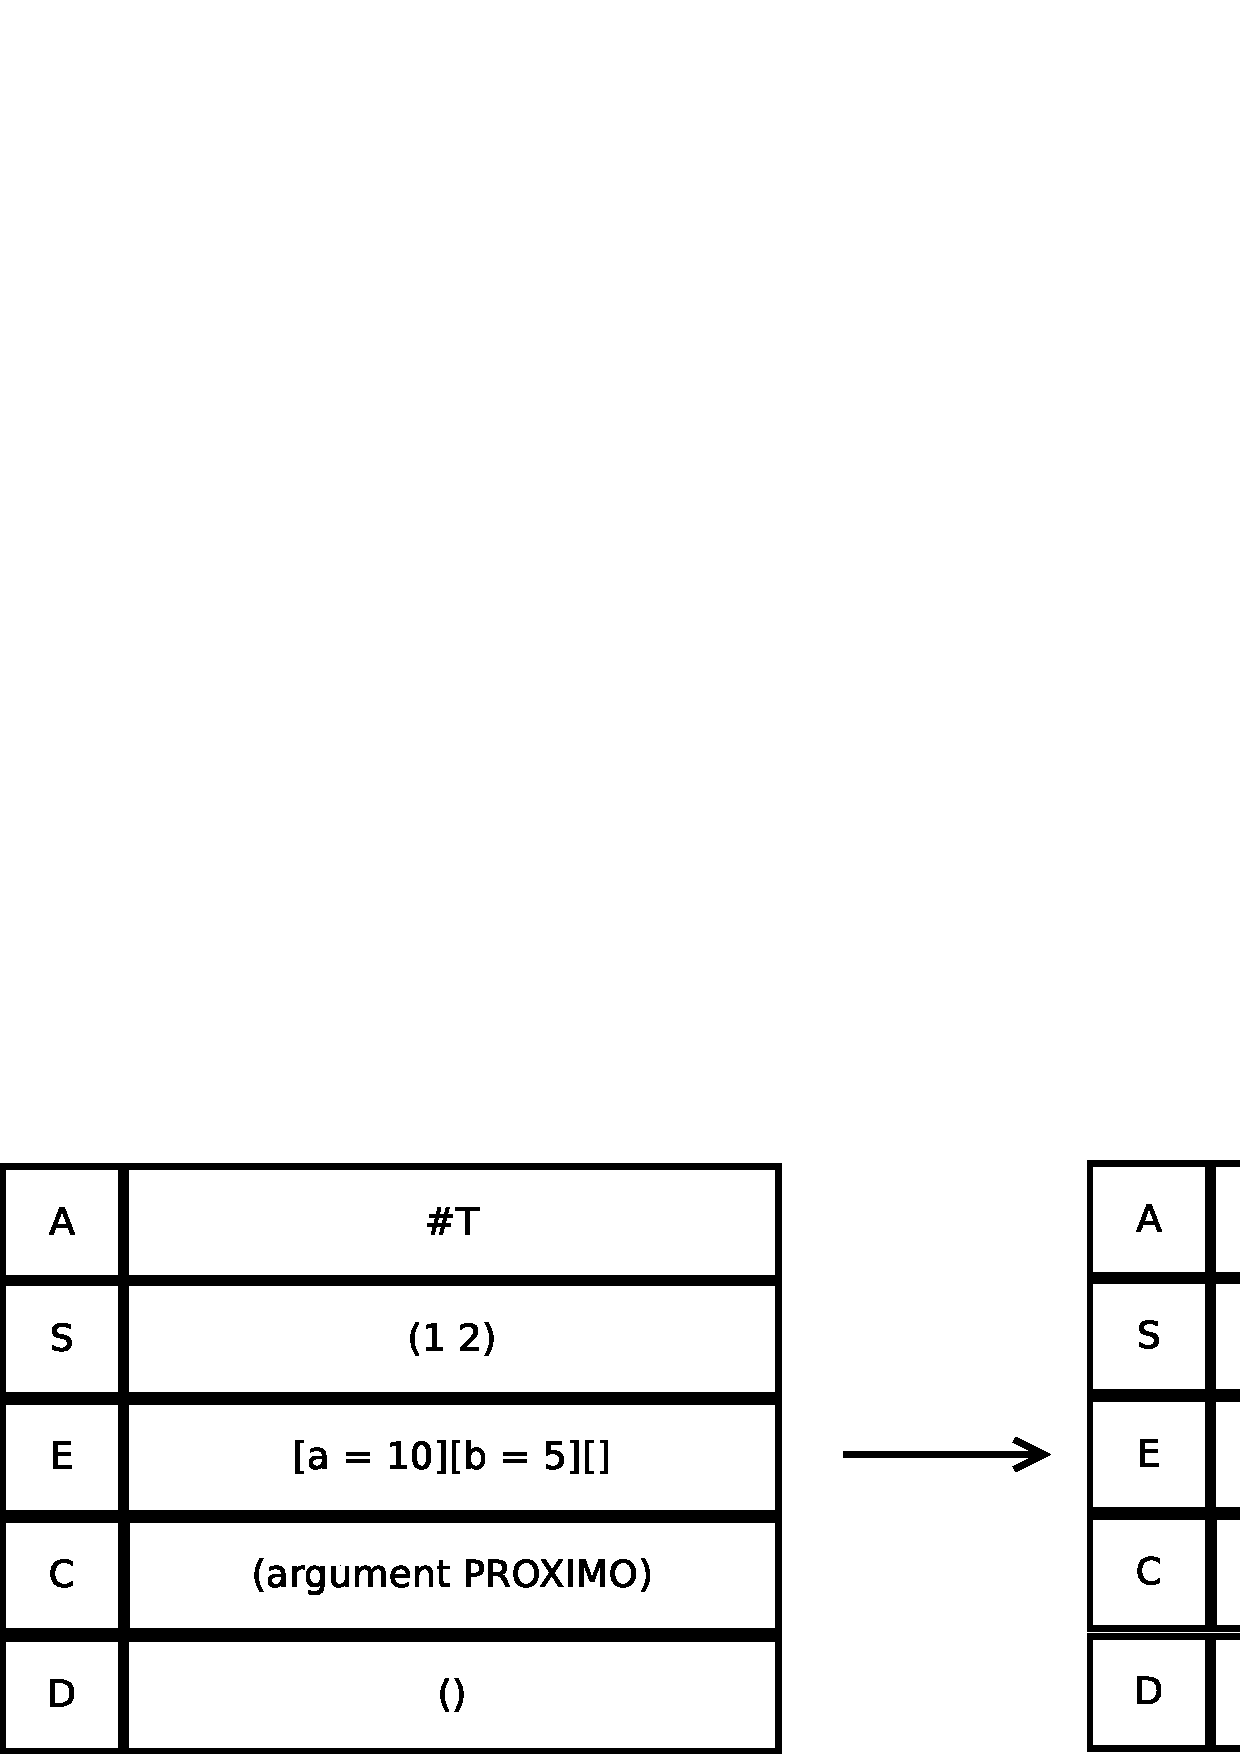
\includegraphics[width=.8\textwidth]{../images/op-argument.pdf}
\caption{Comportamento da máquina ao executar uma instrução \sctt{argument}}
\label{fig:op-argument}
\end{figure}


A instrução \sctt{apply}  inicia uma chamada a uma função ou primitiva e não
recebe parâmetro algum. Utiliza como indicador de qual função ou primitiva a
ser chamado o valor atual do \sctt{acumulador}. Um exemplo de sua execução pode
ser visto na figura \ref{fig:op-apply}. 

Caso o valor no \sctt{acumulador} represente uma primitiva, a instrução
simplesmente passa ao código da primtiiva a lista de parâmetros e mais nada. No
entanto, se o valor no \sctt{acumulador} representar uma função ou closure
definida pelo usuário um novo contexto de escopo baseado no valor dos
argumentos e os parâmetros da função é criado e substitui o valor em
\sctt{environment}, o registrador \sctt{stack} recebe uma lista vazia e o valor
do registrador \sctt{code} é substituido pelo código da função em questão. 

\begin{figure}[h!]
\centering
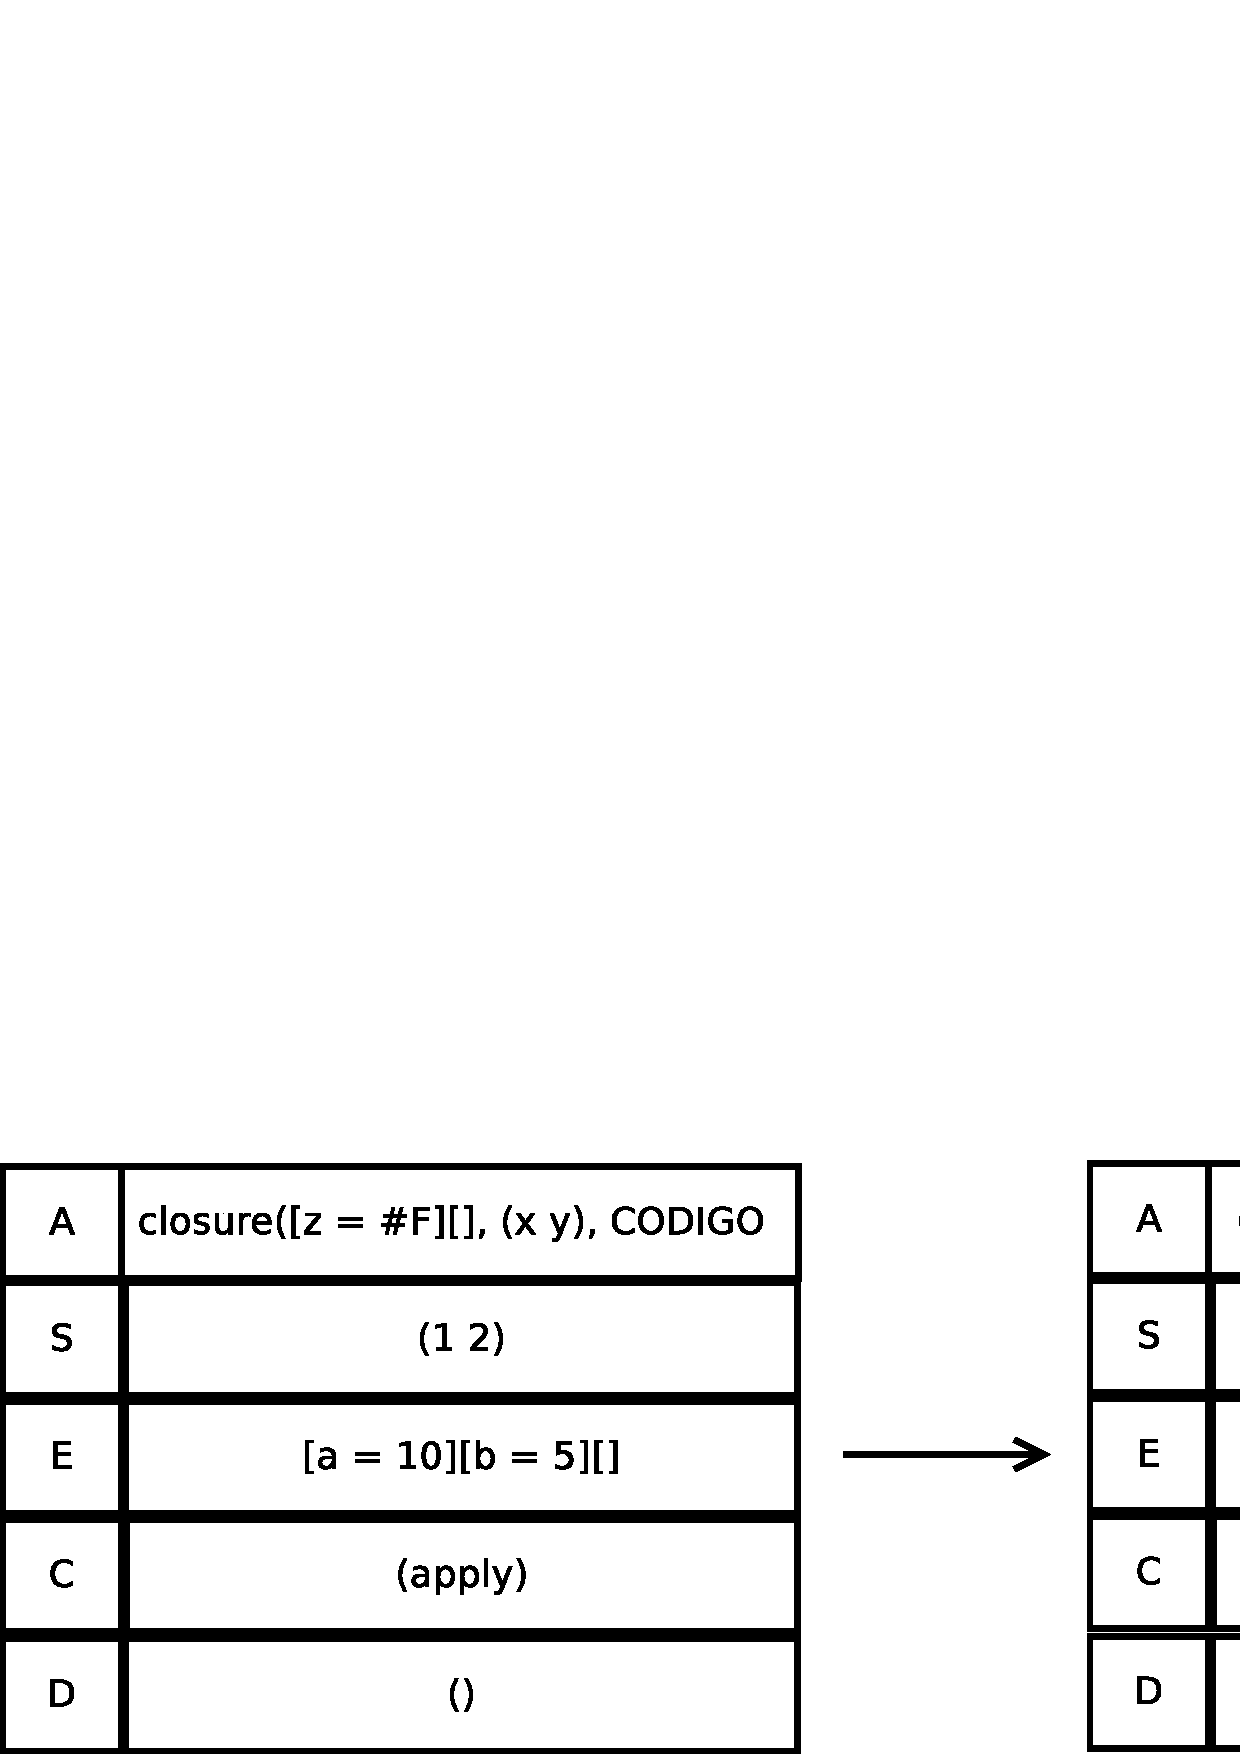
\includegraphics[width=.8\textwidth]{../images/op-apply.pdf}
\caption{Comportamento da máquina ao executar uma instrução \sctt{apply}}
\label{fig:op-apply}
\end{figure}


A instrução \sctt{return}  restaura um frame anteriormente salvo pela instrução
\sctt{frame}. Não recebe parâmetro algum e configura os valores dos
registradores \sctt{stack}, \sctt{environment}, \sctt{code} e \sctt{dump} para
os valores contidos no primeiro elemento da pilha armazenada no registrador
\sctt{dump}. Mantém o registrador \sctt{acumulador} intacto. Um exemplo de sua
execução pode ser visto na figura \ref{fig:op-return}. 

\begin{figure}[h!]
\centering
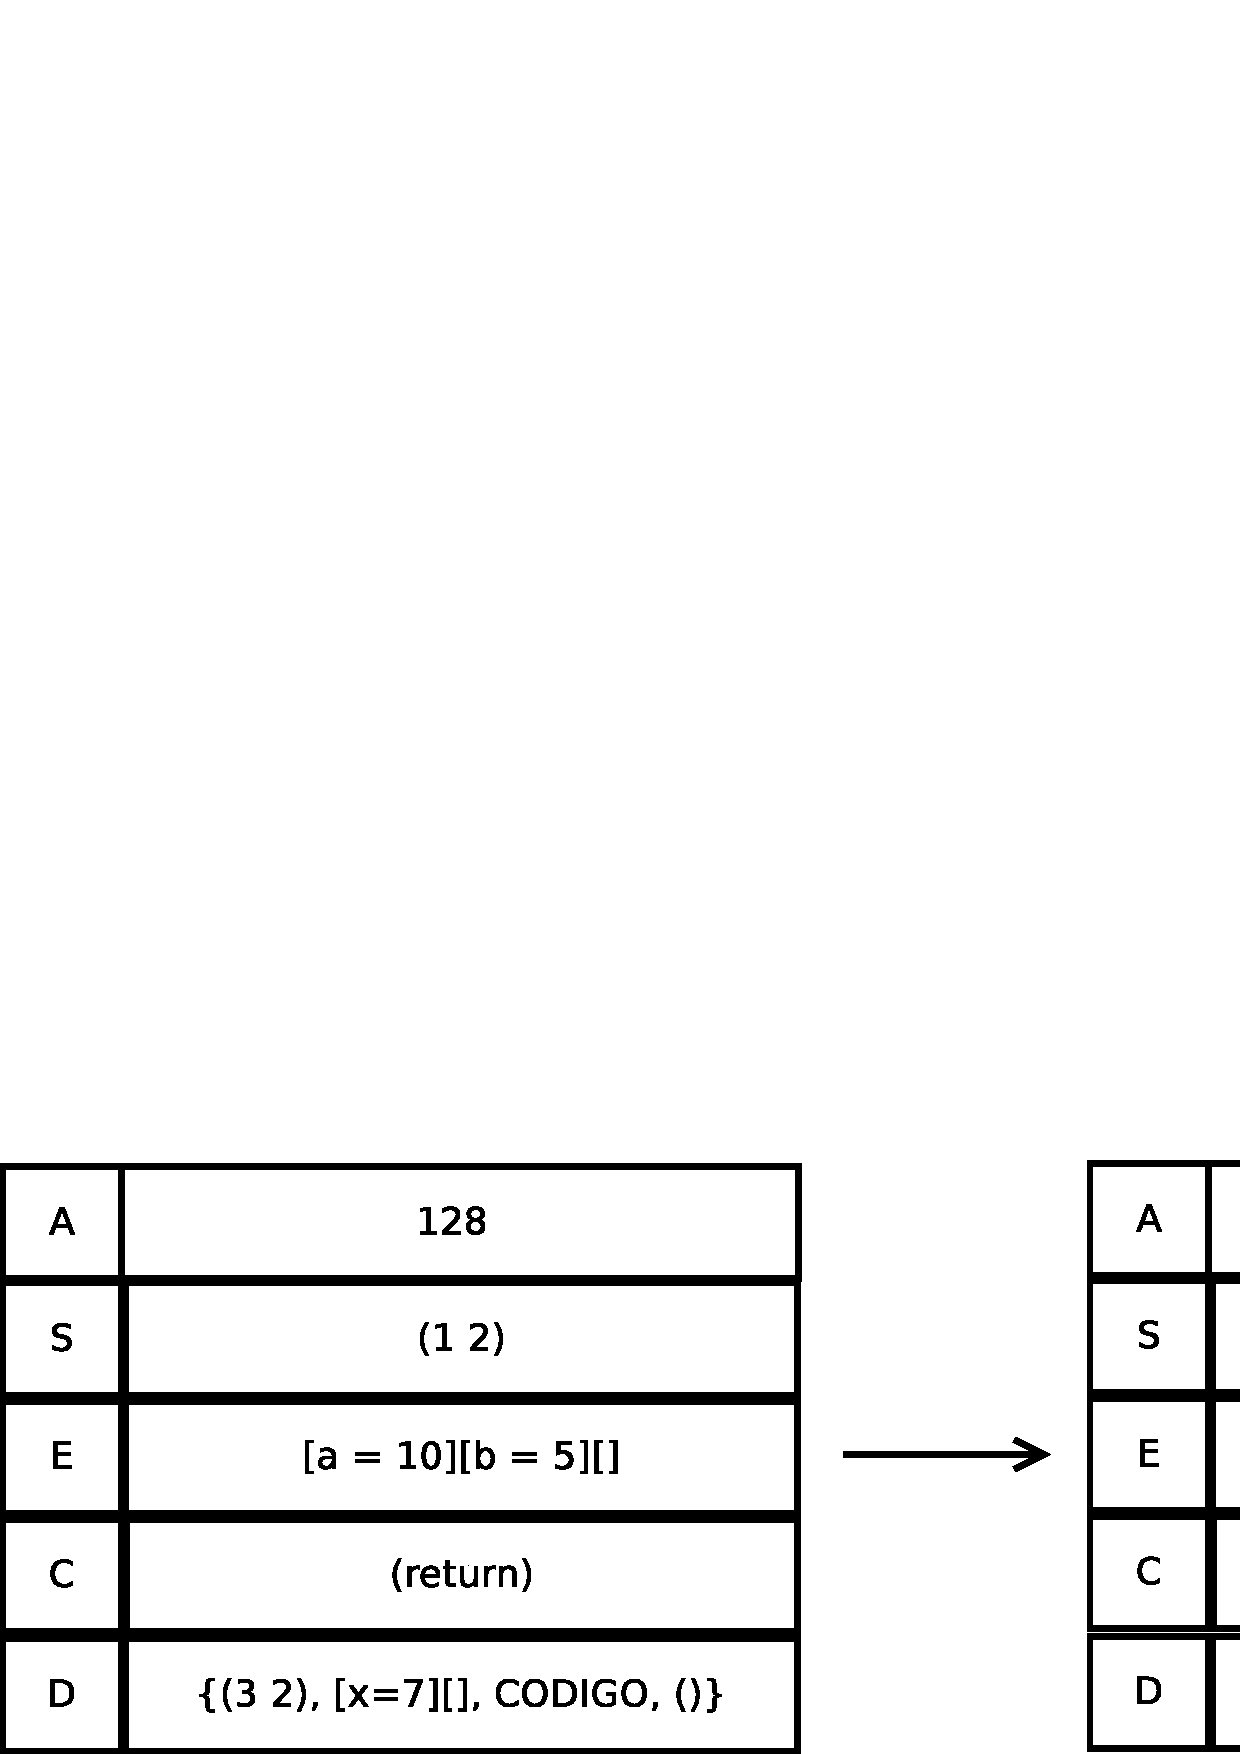
\includegraphics[width=.8\textwidth]{../images/op-return.pdf}
\caption{Comportamento da máquina ao executar uma instrução \sctt{return}}
\label{fig:op-return}
\end{figure}


A instrução \sctt{reify}  é utilizada para restaurar a
computação ao ponto de uma continuação previamente obtida. Recebe como
parâmetros \sctt{dump} e \sctt{valor}, que representam, respectivamente, o
conteúdo do registrador \sctt{dump} no momento da criação da continuação e o
valor a ser restaurado para o \sctt{acumulador} quando a continuação for
restaurada. O efeito final da instrução, é o de retornar ao ponto em que a
continuação foi criada, restaurando os valores presentes no primeiro elemento
da pilha em \sctt{dump}, deixando \sctt{valor} no \sctt{acumulador}. Um exemplo de sua
execução pode ser visto na figura \ref{fig:op-reify}. 

\begin{figure}[h!]
\centering
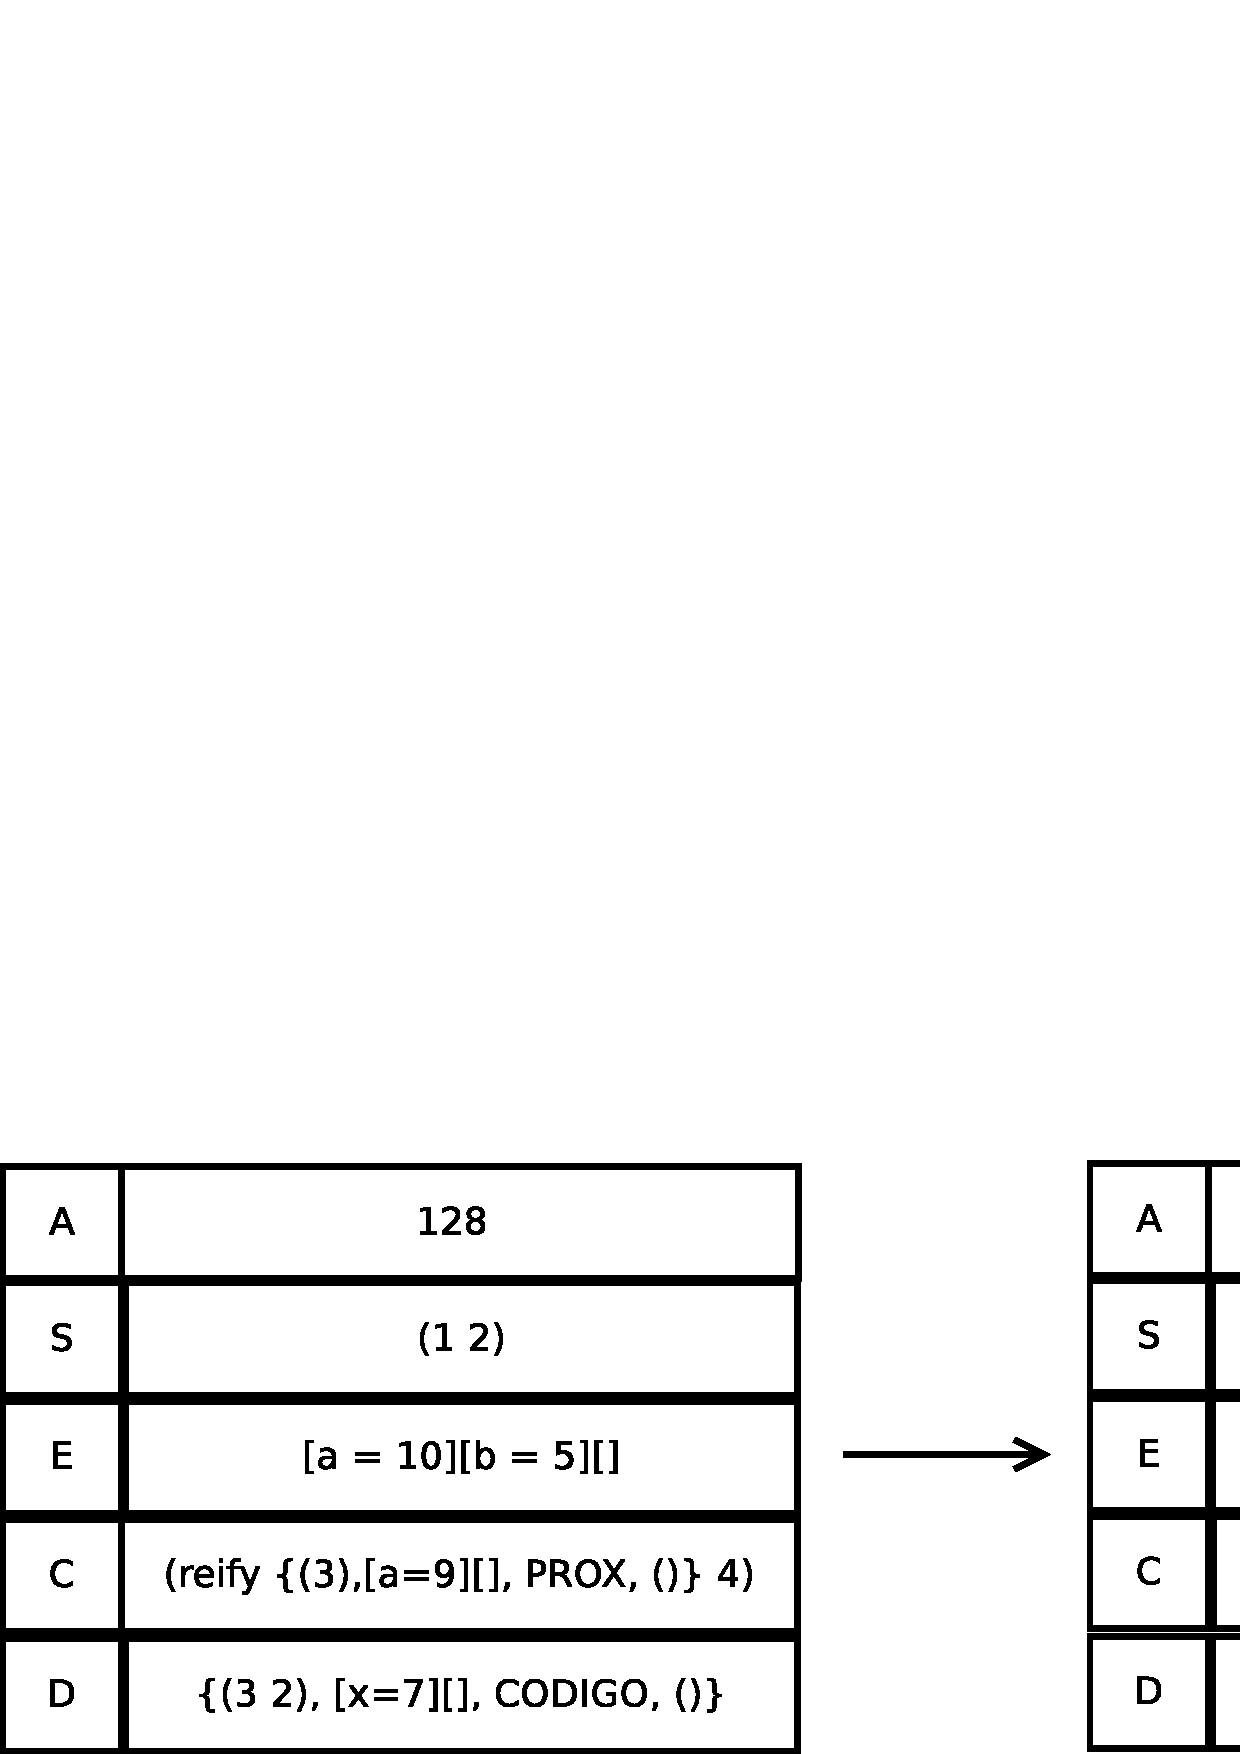
\includegraphics[width=.8\textwidth]{../images/op-reify.pdf}
\caption{Comportamento da máquina ao executar uma instrução \sctt{reify}}
\label{fig:op-reify}
\end{figure}


A instrução \sctt{save}  é responsável por criar uma referência
para a continuação da computação atual. Recebe apenas um parâmetro,
\sctt{próximo}, que é indica qual a próxima instrução a ser executada ao fim
desta. Com a arquitetura utilizada pela máquina virtual, uma continuação é
simplesmente uma closure de apenas um parâmetro, contendo o valor atual do
registrador \sctt{dump} encapsulado, cujo único efeito é chamar a instrução
\sctt{reify} com parâmetros o valor do registrador \sctt{dump} quando a
continuação foi criada e o valor do único parâmetro da closure. Esta closure é
então armazenada no \sctt{acumulador}.

A instrução \sctt{closure}  cria uma nova closure, uma função
em que o contexto na qual foi criada é acessível. Recebe como parâmetros
\sctt{argumentos}, \sctt{corpo} e \sctt{proximo} que são, respectivamente, uma
lista contendo os parâmetros formais da closure a ser criada, o código
compilado do corpo da função e o endereço do código que deve ser executado ao
fim desta instrução. A nova closure criada é armazenada no \sctt{acumulador} e
o registrador \sctt{code} é configurado com o valor de \sctt{próximo}. Um exemplo de sua
execução pode ser visto na figura \ref{fig:op-closure}. 

\begin{figure}[h!]
\centering
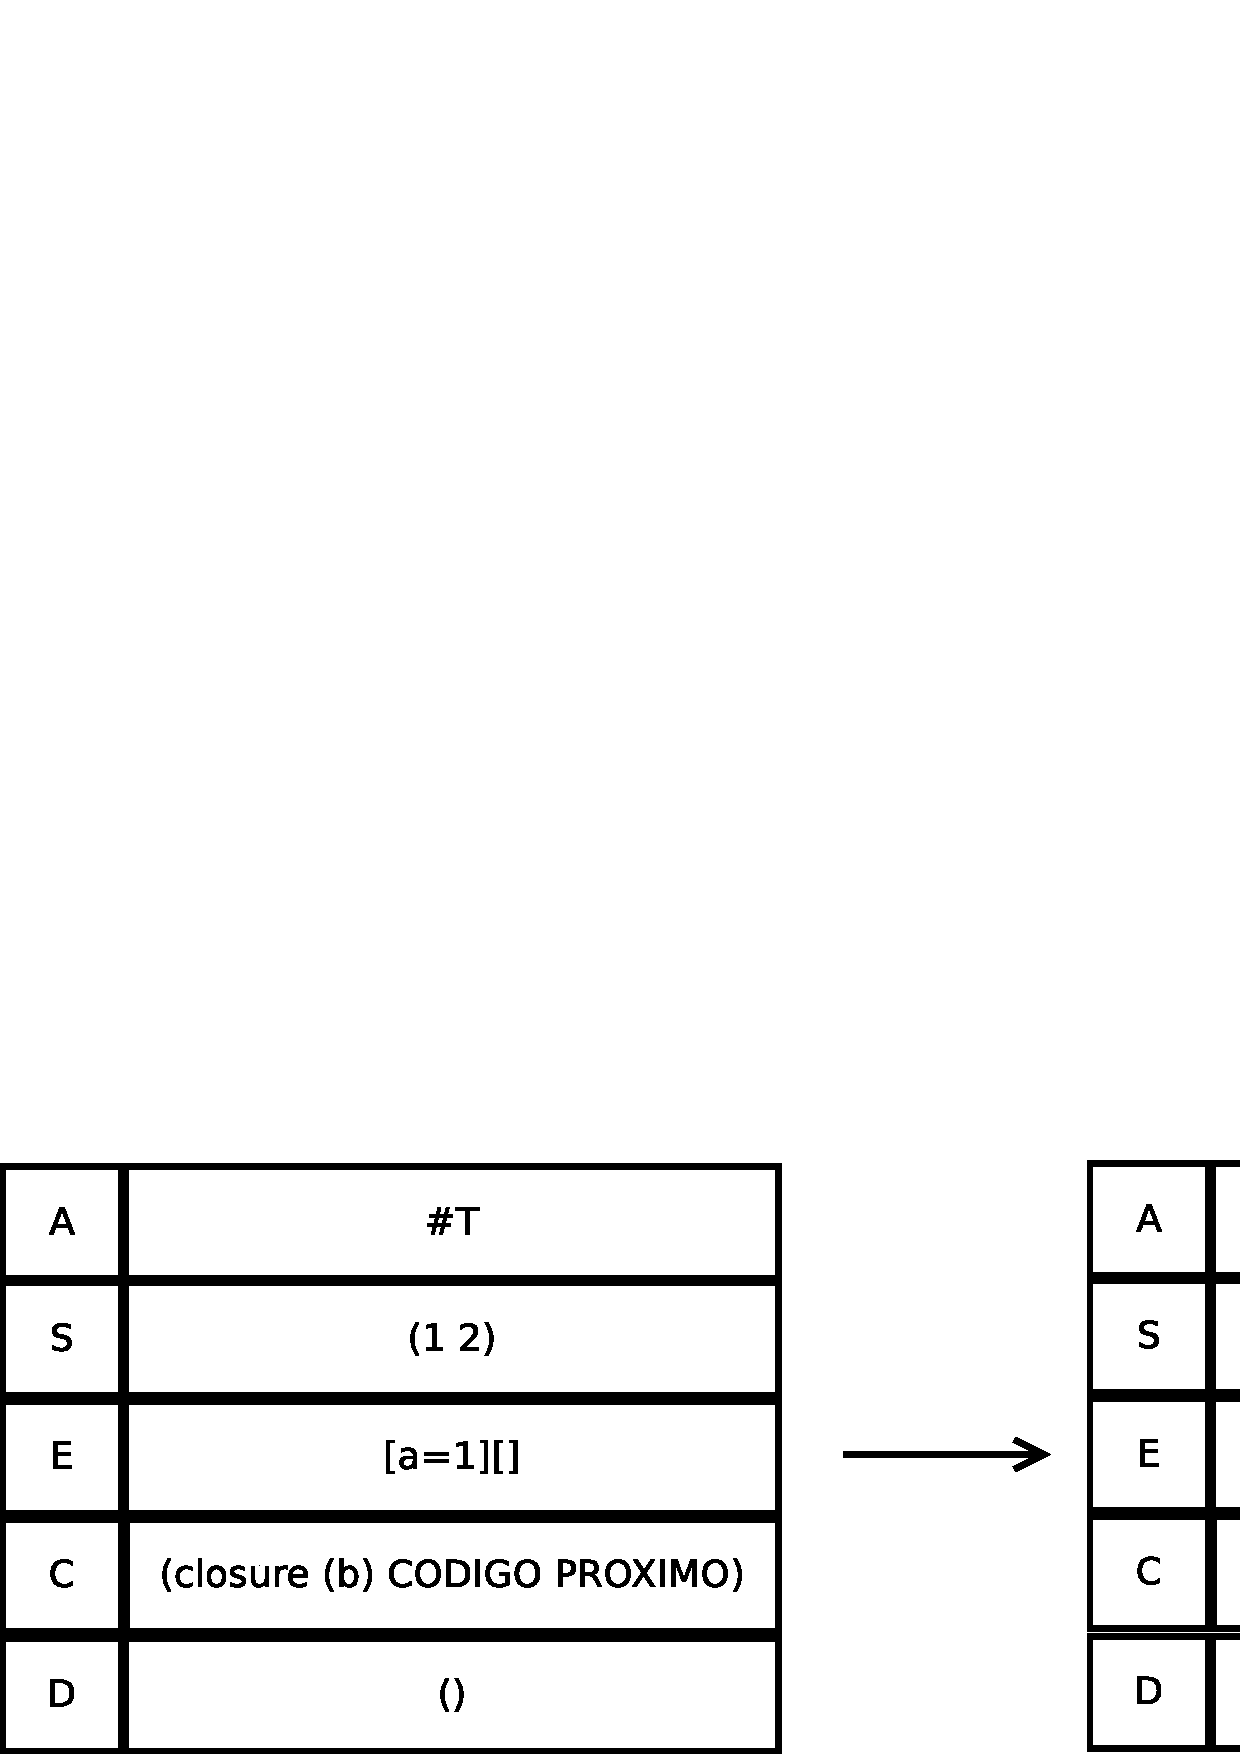
\includegraphics[width=.8\textwidth]{../images/op-closure.pdf}
\caption{Comportamento da máquina ao executar uma instrução \sctt{closure}}
\label{fig:op-closure}
\end{figure}


A instrução \sctt{bind-macro} é uma variante próxima da instrução \sctt{bind},
usada apenas para mitigar uma deficiência do compilador: a falta de um
mecanismo em tempo de compilação para gerenciar macros. Esta instrução recebe
dois parâmetros, \sctt{nome} e \sctt{proximo}, e espera que o \sctt{acumulador}
contenha código para uma macro. Como resultado, guarda em um contexto geral de
macros uma referência para o código da macro sob o nome recebido como
\sctt{nome} e substitui o valor em \sctt{code} pelo valor de \sctt{proximo}.

A última instrução, \sctt{halt}, simplesmente indica à máquina virtual que o
processamento está terminado, e que o valor no \sctt{acumulador} deve ser
retornado como resultado da computação. Não recebe parâmetro algum, e não
altera registrador algum.


